\section{Introduction} 

The construction of the vehicle that our team will present at the
2013 Autonomous Underwater Vehicle (AUV) competition encompasses several new achievements. We explain the
context of our realization by first describing the main
objectives of the competition and how our team is organized.


\subsection{Overview of the Mission}

The objective of the competition is to build an autonomous underwater
vehicle to perform various tasks involving image recognition, and
passive sonar to
interact with its environment. For the vision-guided tasks, the vehicle must 
pass through a validation gate, hit buoys, follow pipes,
pass through set of pipes, drop an object
in a box, launch a projectile through a hexagonal target, and manipulating a wheel.
The sonar tasks consists of
grabbing an object on top of an acoustic pinger and surfacing above it.
The details of the required tasks for the vehicle are described in the
 mission specification on the AUVSI website\footnote[1]{http://www.auvsifoundation.org/foundation/competitions/robosub/}.
Through the design and testing phases, emphasis was placed on
performing a subset of these tasks well rather than attempting all tasks.

\subsection{The Team}
The team consists of twenty members that are divided into three subsystems: mechanical, electronics, and software. In order to maintain a high degree of integration throughout the project, members are encouraged to work in projects that span multiple subsystems. Our hardware is obtained through sponsorship and funding from our university (see Section~\ref{ack}). 

Figure~\ref{organi} illustrates the major components of the AUV
and the reader should refer to it often as we describe the innovative
aspects of those components in the following sections.


\begin{figure*}
\begin{center}
 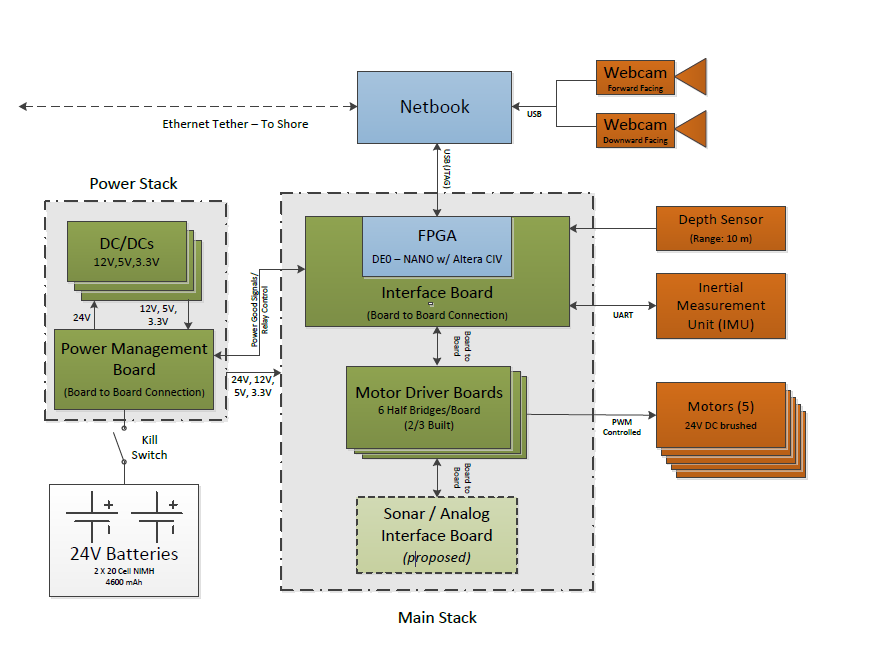
\includegraphics[height=3.3in]{fig/arch.png}
\caption{Organization of the AUV modules and their connectivity.}\label{organi}
\end{center}
\end{figure*}


